\subsection{Optimalno število stolpcev histograma}

Recimo, da ima množica $S$ porazdelitev $P$. Naj bo $p$ gostota verjetnosti te porazdelitve, $h_n$ pa histogram množice $S$ z $n$ stolpci. Velja:
\begin{equation}
    \lim_{\begin{smallmatrix} |S| \to \infty \\ n \to \infty \end{smallmatrix}} h_n(x) = p(x) \quad \text{za} \quad \forall x \in S.
\end{equation}
Histogram je torej lahko ocena gostote verjetnosti množice $S$.

V nobenem vzorcu nimamo na voljo $\infty$ podatkov, zato moramo paziti na izbiro števila stolpcev histograma. Če je $n>|S|$, bo najmanj en stolpec prazen (oz. bo imel višino 0), torej bo to lahko zelo slab približek za gostoto verjetnosti (npr. normalna porazdelitev je povsod večja od 0). Druga skrajnost je, ko izberemo premalo stolpcev in tako izgubimo podatke o porazdelitvi (moduse, če jih ima vzorec več).


\begin{zgled}
Vzemimo množico $S_0 = \{1,1.3,1,2.5,3,3.5,3.6,4,4.1,4.2,5\}$. Poglejmo si histograme ob različni izbiri števila stolpcev.
\begin{figure}[!h]
    \centering
    \begin{subfigure}{0.3\textwidth}
        \centering
        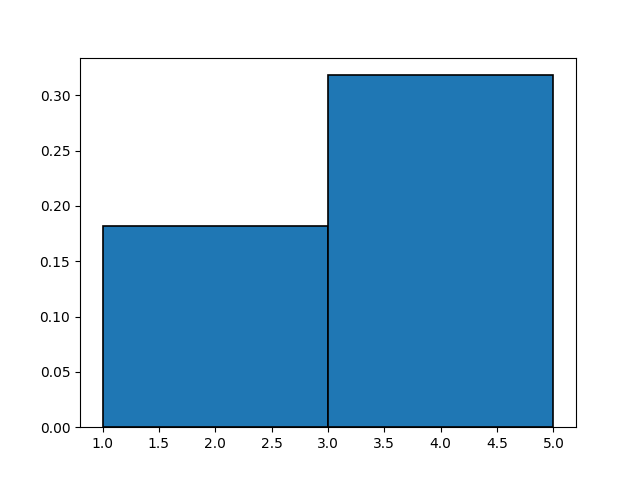
\includegraphics[scale=0.29]{hist-2bina.png}
        \caption{$n=2$}
        \label{2-bina}
    \end{subfigure}
    \begin{subfigure}{0.3\textwidth}
        \centering
        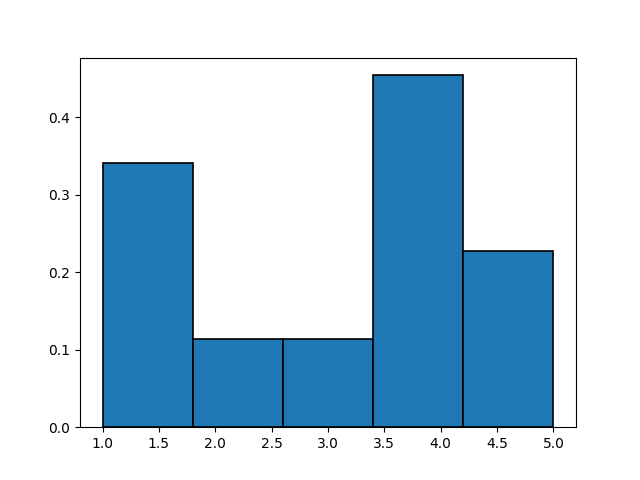
\includegraphics[scale=0.29]{hist-5binov.png}
        \caption{$n=5$}
        \label{5-binov}
    \end{subfigure}
    \begin{subfigure}{0.3\textwidth}
        \centering
        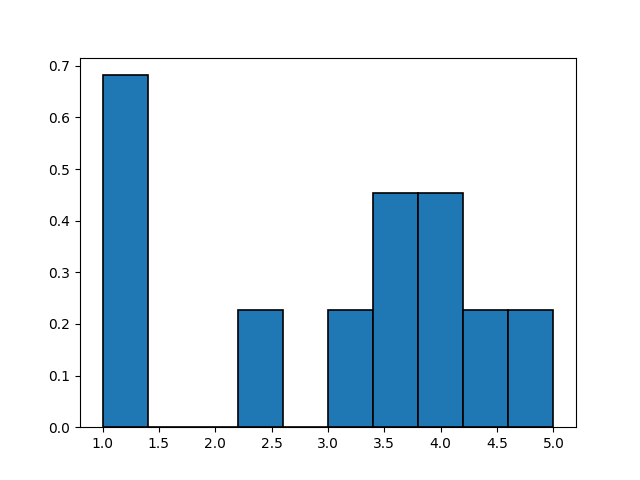
\includegraphics[scale=0.29]{hist-10binov.png}
        \caption{$n=10$}
        \label{10-binov}
    \end{subfigure}
    \caption{Histogrami z različnimi števili stolpcev.}
\end{figure}

V primeru \ref{2-bina} smo izbrali premalo stolpcev, s čimer lahko zgrešimo pomembne lastnosti množice $S$. V primeru \ref{10-binov} pa smo izbrali preveč stolpcev, s čimer dobimo prazne stolpce.
\end{zgled}

Obstaja veliko izbir za optimalno število stolpcev. Naštejmo jih. Za vse izbire naj bo $S$ vzorec in $m = |S|$ moč vzorca.

\pagebreak

\subsubsection{Korenska izbira}
Pri tej izbiri optimalno število stolpcev histograma izračunamo po naslednji formuli:
\begin{equation}
    n = \big\lceil \sqrt{m}\  \big\rceil.
\end{equation}
Izračunamo torej kvadratni koren od števila podatkov v vzorcu in zaokrožimo to število na najmanjše celo število, ki je večje od dobljenega korena.

% preveri alternativo za sklanjanje za Rice.
% PRAVILNO: Riceovo - mi ni všeč
% Kaj, ce je Rice bila zenska? Zaenkrat se izognem sklanjanju
% \subsubsection{Riceovo pravilo}
\subsubsection{Rice}
Pri tej izbiri optimalno število stolpcev za histogram izračunamo na naslednji način:
\begin{equation}
    n = \big\lceil \sqrt[3]{m}\  \big\rceil.
\end{equation}

\subsubsection{Sturges}
Pri tej izbiri optimalno število stolpcev izračunamo po naslednji formuli:
\begin{equation}
    n = \big\lceil \log_2{m}\  \big\rceil + 1.
\end{equation}
Ta formula je zelo varčna, saj logaritem narašča zelo počasi. Medtem ko bo pri korenski izbiri in 10000 podatkov optimalno število stolpcev 100, bo pri Sturgesovi formuli število stolpcev enako 11.

Vse tri do zdaj naštete izbire delujejo zelo naivno, saj upoštevajo le velikost vzorca, ne pa ostalih njegovih lastnosti, npr. variance. Kljub temu pa se izkaže, da te metode zelo dobro konkurirajo z ostalimi, če gledamo lepe porazdelitve, npr. normalne porazdelitve. Težava so bolj kompleksne porazdelitve, ki imajo visoke repe in so na eni strani omejene. Pri teh hitro dobimo premalo stolpcev in moramo nujno upoštevati še kakšno drugo lastnost, ne le velikosti vzorca.

\pagebreak
Poglejmo si sedaj še izbiri, ki upoštevata bolj specifične lastnosti vzorca. Ti dve formuli sicer vrneta optimalno širino stolpca, a zlahka iz tega podatka dobimo optimalno število stolpcev (glej formulo \eqref{sirina_stevilo}). 

\subsubsection{Scoot}
Formula Scoot poleg velikosti vzorca upošteva še njegov standardni odklon $\sigma$:
\begin{equation}
    h = 3,49 \cdot \sigma \cdot m^{-1/3}.
\end{equation}

\subsubsection{Freedman-Diaconis}
Ta izbira prav tako uporabi še dodatno lastnost poleg velikosti vzorca, in sicer medkvartilno razdaljo vzorca $IQR$ (angl. \textit{interquartile range}), to je razlika med zgornjim in spodnjim kvartilom. 
\begin{equation}
    h = 2 \cdot IQR \cdot m^{-1/3}.
\end{equation}

Ker smo že sproti opisali izbire, primer izpustimo. Omenimo pa, da sta zadnji dve metodi v splošnem najboljši, saj poleg velikosti vzorca upoštevata še dodatne lastnosti vzorca, poleg tega pa je izračun variance in medkvartilne razdalje hiter, zato metodi nista časovno potratni.